\documentclass[conference]{IEEEtran}
\IEEEoverridecommandlockouts
\usepackage{cite}
\usepackage{amsmath,amssymb,amsfonts}
\usepackage[
    bookmarks=false,         % Fixes 'bookmarks' error
    draft,                   % Fixes 'links' error by disabling hyperlinks
    pdfborder={0 0 0}
]{hyperref}
\usepackage{xurl}       
\urlstyle{same}  
\usepackage{algorithmic}
\usepackage{graphicx}
\usepackage{textcomp}
\usepackage[acronym]{glossaries}
\usepackage{xcolor}
\usepackage{multirow}
\usepackage{booktabs}
\usepackage{url}
\usepackage{algorithm}
\usepackage{algpseudocode}
\usepackage{tikz}
\usetikzlibrary{positioning, calc, shapes.geometric}
\tikzset{
    block/.style={draw, fill=blue!5, text width=2.8cm, align=center, minimum height=1cm, font=\small},
    branch/.style={draw, fill=gray!5, text width=2.5cm, align=center, minimum height=0.8cm, font=\small},
    arrow/.style={thick,->,>=stealth}
}

\usepackage[acronym]{glossaries}
\makeglossaries
\newacronym{dl}{DL}{Deep Learning}


\def\BibTeX{{\rm B\kern-.05em{\sc i\kern-.025em b}\kern-.08em
    T\kern-.1667em\lower.7ex\hbox{E}\kern-.125emX}}

\title{\LARGE \bf
    Avena Road Side: Modernizing In-Situ Pavement Monitoring and Asset Management\squeezeupaftertitle%
}

\author{
     Anuska Das, Andrew~D.~Balmos, Boonam Shin, James~V.~Krogmeier, and Yaguang Zhang\squeezeupafterauthors% 
    \thanks{
        This study is supported by the Joint Transportation Research Program (JTRP) between the Indiana Department of Transportation (INDOT) and Purdue University. The study is funded by State Planning & Research (SPR) project SPR-4918 "Enhancing Pavement Instrumentation and Monitoring: A Novel Edge First, Network-Level Solution for Pavement and Roadside Sensors with Live Data Visualization"}%
}

\begin{document}

\maketitle
\thispagestyle{empty}
\pagestyle{empty}

\begin{abstract}
The effective management of highway infrastructure relies on robust pavement health monitoring, yet traditional methods suffer from sparse, reactive data and high operational costs. Current in-situ sensor deployments, while valuable, often lack real-time context and necessitate cumbersome manual data collection, hindering predictive maintenance. This paper introduces Avena: Road Side (AvenaRS), an open-source, edge-computing-enabled telemetry system designed for continuous, high-fidelity pavement monitoring in remote, network-constrained environments. AvenaRS integrates diverse subsurface sensors with a real-time vision system to capture dynamic vehicle characteristics (e.g., speed, position, weight) for contextualizing and normalizing sensor responses. Leveraging the Avena framework and NATS messaging queue, the system processes high-rate sensor and video data at the edge, optimizing bandwidth by intelligently routing only relevant information to a central node. Furthermore, a solar-powered and battery-backed design ensures continuous operation independent of grid infrastructure. Through a detailed system overview, we demonstrate AvenaRS's capacity for unattended, 24/7 data collection and its ability to transform sensor signals into actionable insights. This work provides a scalable and cost-effective solution for proactive pavement management, enabling a deeper understanding of traffic-induced wear and facilitating data-driven decision-making for sustainable infrastructure.

\end{abstract}

\begin{IEEEkeywords}
Pavement monitoring, edge computing, traffic monitoring, roadside telemetry, subsurface sensors, data acquisition, computer vision, infrastructure health monitoring, smart highways

\end{IEEEkeywords}

\section{Introduction and Motivation}
Monitoring pavement health is an essential activity for transportation agencies~\cite{Barriera2020SituPavementMonitoring}. It ensures safe and sustainable highway infrastructure. Departments seek to leverage data-driven allocation processes that optimize the distribution of their limited resources for building, rehabilitating, and reconstructing public roadways across the entire network~\cite{Jha2023DataDrivenWeb}. Traditional measurement techniques include manual scouting, core drilling, laser surface scanning, International Roughness Index (IRI), Falling Weight Deflectometer (FWD), and Ground Penetrating Radar (GPR) measurements~\cite{Xin2025}. However, these methods come with a significant burden of complex logistics, labor costs, and traffic control, which limits the quantity of testing that can be accomplished. Perhaps even more importantly, these constraints severely limit the data available for decision-making, forcing infrastructure management decisions to be based on insufficient information.

To limit labor and traffic disruption, there has been an increased demand to include pavement health instrumentation during the road construction phase~\cite{Xue2014PavementHealthMonitoring, Alavi2016Continuoushealthmonitoring,Ceylan2016FieldDemo, Micko2023}. As an example, pressure cells, strain gauges, soil moisture, and temperature sensors can be embedded within the pavement and engineered sub-grade layers~\cite{TenorioFilho2023}. Changes in how pressure and strain propagate through the layers of the road section can inform how pavement ages and indicate sources of failure, particularly in response to dynamic loads such as full-speed traffic, slow or stopped traffic, and heavy vehicles~\cite{Heller2023}.

Typically, these in-situ sensors include long signal cables routed in conduit underground to a protected, roadside cabinet~\cite{Liu2024SensorBasedStructural,Ye2024}. This allows agency employees to bring measurement equipment to the sensor cabinet and collect data in a safe location, without traffic management. While this represents a massive reduction in many burdens of collecting data, including enabling collection campaigns under live load conditions, it does not fully address the timeliness issue. A human operator must physically transport sensitive data collection devices to each instrumented road section whenever data collection is required.
In addition, this operator must carefully coordinate data collection with anticipated traffic levels and weather conditions to both capture the environmental factors of interest and ensure operator safety during roadside access. Essentially, these instrumented road sections still serve a limited utility in the development of predictive maintenance programs.

This paper proposes an alternative cost-effective and open-source solution built upon the Avena \cite{avena2022} software framework. Our solution, called Avena Road Side (AvenaRS), continuously monitors instrumented pavement down to individual vehicle loading events, in all conditions and traffic loads. It features connectivity capabilities that allow for remote configuration, control, and data access. In the following sections, we will detail how this system will continuously collect, share, and store high-fidelity sensor data. This includes additional enriching metadata such as vehicle position, velocity, and weight class estimation via an onboard camera system. All of this is accomplished by leveraging local edge computing capabilities that process the incoming data in real-time. We also discuss the design of a solar subsystem and the tradeoffs that may be required in practice, considering the realities of low-light winters.


\section{Avena Road Side: System Overview}
To effectively monitor changes in pavement performance, it is critical that year-over-year sensor data be properly conditioned for comparison.
In live traffic situations, many factors must be accounted for to ensure this comparability.
While fundamental changes in ground sensors may not occur between data collections, the loading events are caused by the traffic itself.
Vehicle speeds, accelerations, weights, and tire positions are critical factors that influence the expected embedded sensor readings.
AvenaRS was built to capture not just the sensor data but also the necessary metadata to make such compensations.
\begin{figure}[!ht]
    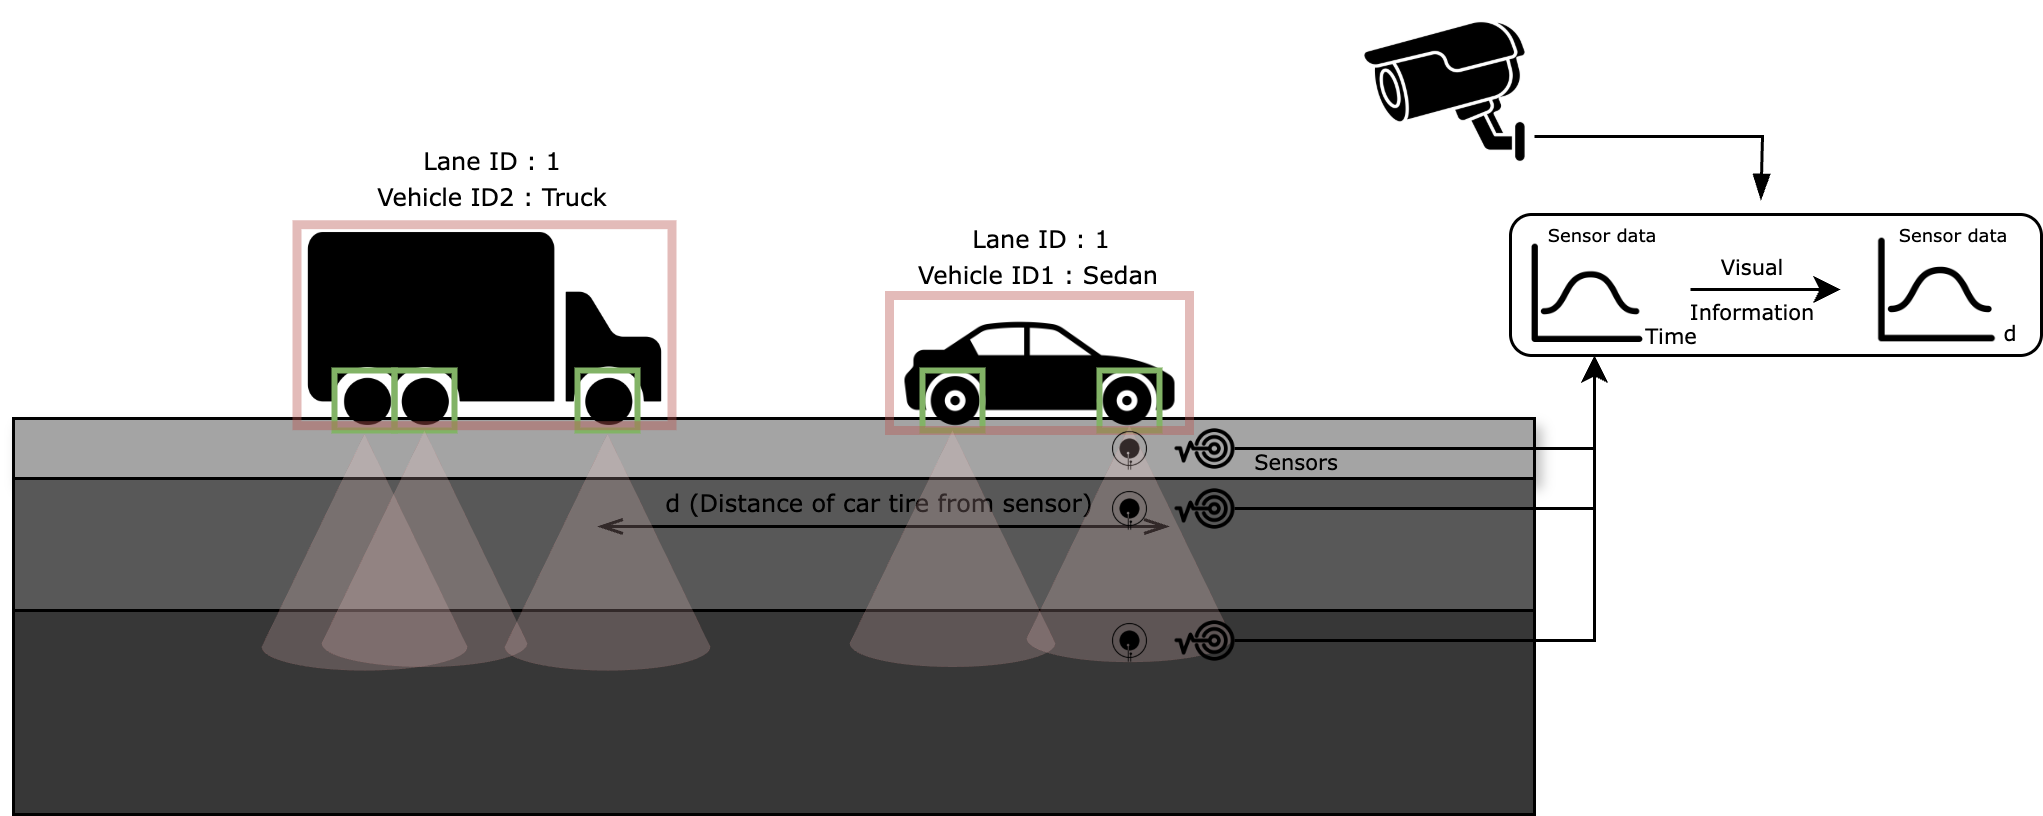
\includegraphics[width=\textwidth]{figures/Camera_sys.png}
    \caption{A graphical depiction of the AvenaRS system.}
    \label{fig:camera-sys}
\end{figure}
As shown in Figure~\ref{fig:camera-sys}, each vehicle applies stress to the pavement.
As this stress transfers through the pavement sub-layers, it also spreads out, reducing the overall load per unit area.
These pressure "cones" move with the vehicle and are precisely what the embedded sensors are intended to observe.
However, the sensor data is captured at a constant rate in the time domain, regardless of how fast the approaching vehicle is traveling.
Therefore, AvenaRS deploys a vision system capable of tracking vehicles and estimating the necessary parameters, such as vehicle velocity, to undo these effects.
This allows the recorded time-domain signal to be transformed into a "distance" domain parameterized by the surface distance between the loaded vehicle's tire and the sensor position.
When all load events are brought into this same distance domain, they become comparable without regard to velocity.
Similarly, vehicle acceleration and weight play important roles, which the vision system also works to estimate for use in data normalization.

Finally, AvenaRS was built with a state-wide road network in mind from the beginning.
An agency has more than one pavement section to monitor across its highly distributed roadway network.
To support this need, AvenaRS was built such that every instrumented road section, while paired with a complete and standalone edge AvenaRS installation, also seamlessly participates in a network-wide system powered by the Avena framework.

\begin{figure}[!ht]
    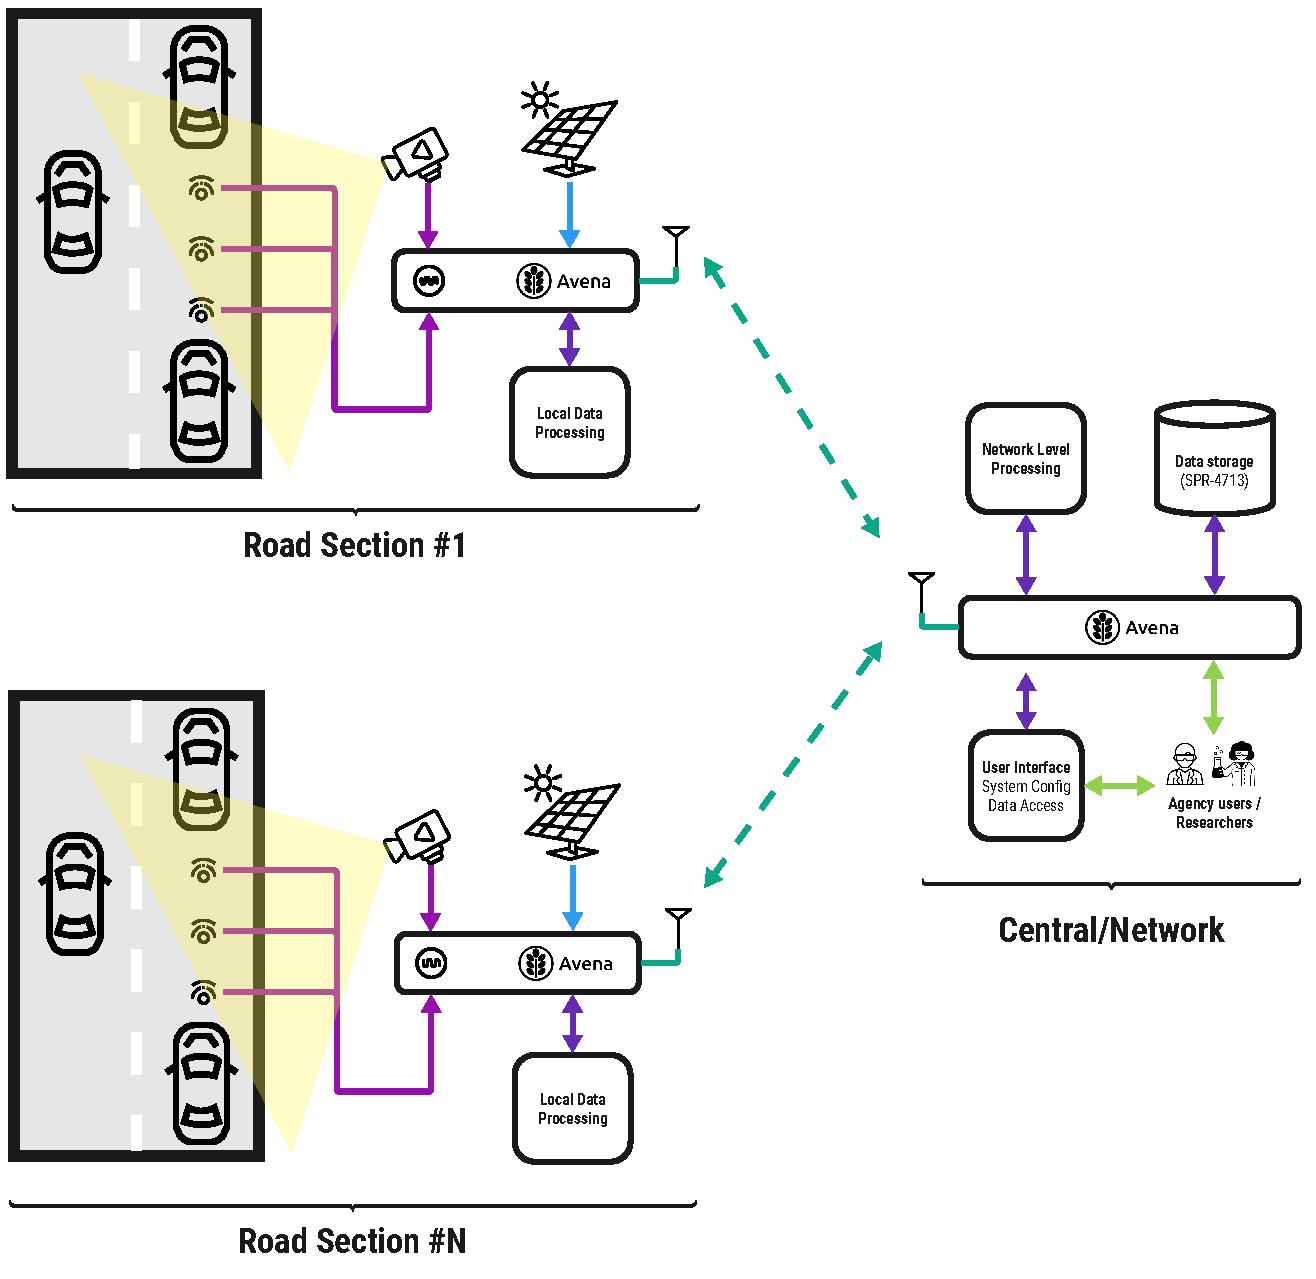
\includegraphics[width=0.8\textwidth]{figures/AvenaRS.pdf}
    \caption{Individual AvenaRS devices participating in a network wide system.}
    \label{fig:concept-arch}
\end{figure}

As shown in Figure~\ref{fig:concept-arch}, the overall AvenaRS architecture consists of many AvenaRS devices connecting back to a central node.
This central node can pull data streams from and transmit command and control signals to an arbitrary number of units.
Agency employees and researchers use this central installation to configure each section's monitoring system and to access the collected data.

\section{Avena Road Side: System Overview}
To effectively monitor changes in pavement performance, it is critical that year-over-year sensor data be properly conditioned for comparison.
In live traffic situations, many factors must be accounted for to ensure this comparability.
While fundamental changes in ground sensors may not occur between data collections, the loading events are caused by the traffic itself.
Vehicle speeds, accelerations, weights, and tire positions are critical factors that influence the expected embedded sensor readings.
AvenaRS was built to capture not just the sensor data but also the necessary metadata to make such compensations.

\begin{figure}[!ht]
    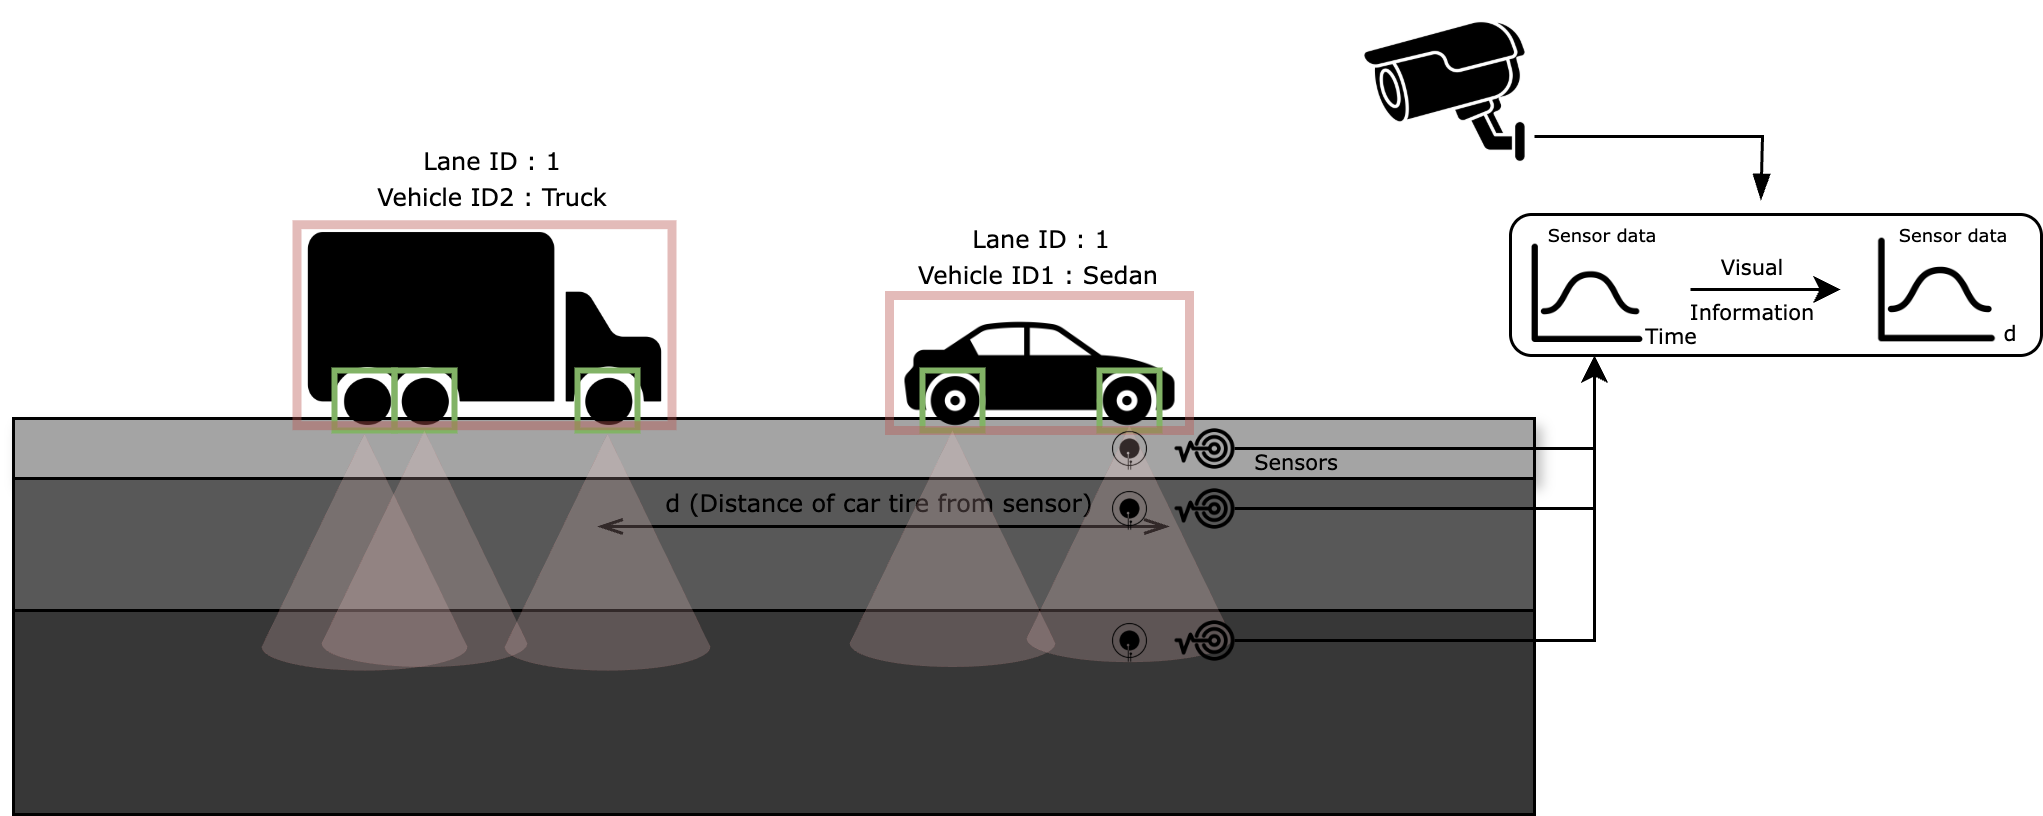
\includegraphics[width=\textwidth]{figures/Camera_sys.png}
    \caption{A graphical depiction of the AvenaRS system.}
    \label{fig:camera-sys}
\end{figure}

As shown in Figure~\ref{fig:camera-sys}, each vehicle applies stress to the pavement.
As this stress transfers through the pavement sub-layers, it also spreads out, reducing the overall load per unit area.
These pressure "cones" move with the vehicle and are precisely what the embedded sensors are intended to observe.
However, the sensor data is captured at a constant rate in the time domain, regardless of how fast the approaching vehicle is traveling.
Therefore, AvenaRS deploys a vision system capable of tracking vehicles and estimating the necessary parameters, such as vehicle velocity, to undo these effects.
This allows the recorded time-domain signal to be transformed into a "distance" domain parameterized by the surface distance between the loaded vehicle's tire and the sensor position.
When all load events are brought into this same distance domain, they become comparable without regard to velocity.
Similarly, vehicle acceleration and weight play important roles, which the vision system also works to estimate for use in data normalization.

Finally, AvenaRS was built with a state-wide road network in mind from the beginning.
An agency has more than one pavement section to monitor across its highly distributed roadway network.
To support this need, AvenaRS was built such that every instrumented road section, while paired with a complete and standalone edge AvenaRS installation, also seamlessly participates in a network-wide system powered by the Avena framework.

\begin{figure}[!ht]
    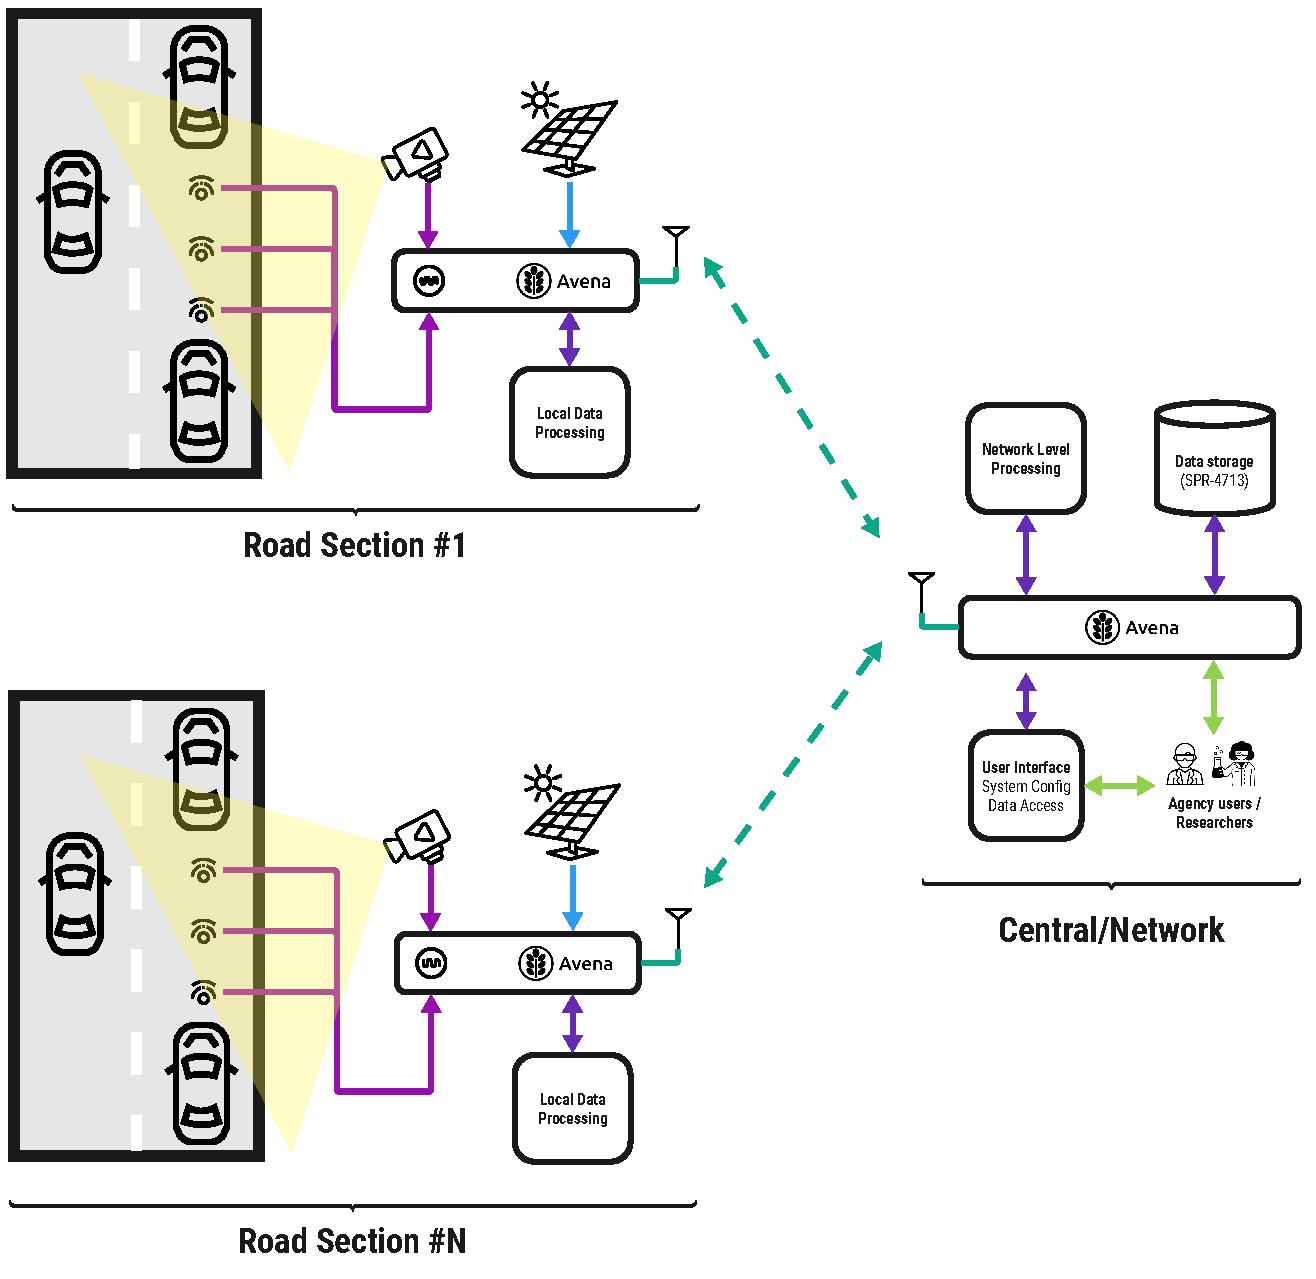
\includegraphics[width=0.8\textwidth]{figures/AvenaRS.pdf}
    \caption{Individual AvenaRS devices participating in a network wide system.}
    \label{fig:concept-arch}
\end{figure}

As shown in Figure~\ref{fig:concept-arch}, the overall AvenaRS architecture consists of many AvenaRS devices connecting back to a central node.
This central node can pull data streams from and transmit command and control signals to an arbitrary number of units.
Agency employees and researchers use this central installation to configure each section's monitoring system and to access the collected data.

\subsection{Embedded Pavement Sensors and Data Acquisition}
Pavement performance is measured by sensor suites comprised of a combination of earth pressure cells, horizontal and vertical strain gauges, soil compression gauges, soil moisture sensors, and temperature sensors.
Each sensor plays a role in determining how forces are transferred from a vehicle through the various pavement layers and into the earth.
AvenaRS provides a means of monitoring changes in these signals' overall tendencies, as well as jointly during dynamic loading events.
Such changes provide insights into pavement behavior, enabling both detection of deterioration and prediction of future maintenance needs.

The acquisition system used by the edge computer is a high sample rate, multi-channel analog front end that allows for simultaneous measurements of many subsurface sensors.
Sensor cabling routes back to the roadside equipment cabinet and connects to open design interface circuit created by the project.
These circuits map the expected sensor signal to the full-scale resolution of the voltage samplers.
The LabJack T7 OEM \cite{labjack_t7_datasheet} is the project's primary voltage sampler; however, discrete analog-to-digital converters may sometimes be used to measure mostly static sensors, like soil temperature.
For sensors that require differential inputs, such as analog earth pressure cells and strain gauges, an differential preamplifier is provided in the interface circuit, and corrected for post-process data calibration.

The maximum sample rate supported by the LabJack T7 is 100 kilo-samples per second. 
However, to reduce costs, multiple sensors can be multiplexed onto a single sampler, thereby reducing the total number of LabJacks needed.
This has the effect of reducing the per-sensor maximum sample rate, but the relatively slow pavement responses typically require no more than 10 kilo-samples per second to adequately capture.
Therefore, AvenaRS plans for roughly 10 total sensors per LabJack device.

At this reduced rate of 10 kilo-samples per second, per channel, and assuming that each sample is recorded as a 4-byte floating-point number, the projected data size is roughly 3.2 GB per channel per day.
To balance this high-fidelity, but large data, with the practical storage and transmission constraints of roadside embedded hardware, AvenaRS will support per-channel, reduced sampling rates down to sub-hertz.
The edge computing capabilities allow for this downscaling from the full resolution to occur only during non-loading events, preserving the full response details during true pavement responses, considerably reducing the overall storage requirements.

Finally, some popular sensors on the market provide a fully digital data interface.
For example, it is somewhat typical to find soil moisture sensors that rely on the SDI-12 communication protocol.
To support such digital sensors, AvenaRS also deploys a microcontroller powered subsystem that can poll digital serial buses for data and forwarded the results into the AvenaRS system to be available alongside voltage-based sensor data.

\section{Vision Cameras and Vehicle Tracking}

\section{Edge Computing: The Avena Framework}

AvenaRS is powered by the open-source edge computing framework Avena \cite{avena2022, gowda2025enhancing, castiblanco2024avena, castiblanco2024oatsmobile}.
It was developed to encourage the democratization of edge computing hardware and software.
This approach fosters an increase in equipment reuse and interoperability, as it allows different industry players to create and load software on commodity hardware options.
These features are important given that AvenaRS seeks to be not only a robust roadside data collection system, but also a platform for future research and technology development.
Avena itself is based on a deep stack of other open-source technology.
At its core is the Linux operating system, which supports Podman \cite{husain2023analysis} containers to securely run user software directly on the device.

In the context of AvenaRS, the system software running on the edge devices comprises services that manage data acquisition, processing, and storage, such as the LabJack data acquisition system, SDI-12 sensor bus, video cameras, and cellular modems for time reference.
These services continuously read, format, and write data to the Avena network.
As new technology and algorithms are developed by the AvenaRS team or independent third parties, they can be easily deployed alongside the core software.
The device owner can grant them permission to access and create data streams.
Therefore, AvenaRS functions not only as an agency data platform, but also as an instrument for live system testing and research without jeopardizing the core data collection mission or requiring separate investments.

\subsection{Avena Messaging: NATS core} 
Inter-process and inter-device communication within AvenaRS is primarily accomplished via the NATS messaging system, which includes both core NATS functionality and its persistent streaming layer, NATS Jetstream.

NATS core messaging is a simple, yet flexible, open-source message queue that requires low resources, allowing it to run directly on each edge device.
All data, command, and control messages first flow through this local NATS instance, before going anywhere else.
This instance then delivers those messages to any other Avena application that has registered interest, and leaving the rest behind.
As a result, application code does not need to worry about where it's data should go.
It simply gives it the Avena network, and the network decided where and how to route it.
For subscribing applications running on the same edge device, the data does not leave; instead, it is efficiently delivered using the local network stack.
For applications running on other edge devices, in the cloud, or on user equipment, messages are routed over any available network connection.

If the requesting software is not running on the edge device itself but does have a direct networking path, for example, a technician's laptop connected to the AvenaRS Ethernet switch, the data is routed over that direct path to the subscribing program.
For external data subscriptions, messages are first routed to a cloud or centralized NATS instance and then on to the subscribing consumer.
The reason for this is to limit the number of times a single data flow has to be repeated over the potentially expensive cellular or non-terrestrial network-connected radio.
Once the stream has made it to the cloud, it can be routed from there to all interested parties directly.
However, in the case that a central instance is unavailable due to an outage or lack of edge connectivity, external software can always request data directly from the edge device assuming there is some sort of connectivity between the two nodes.
This has the side effect of greatly increasing overall availability, but often trades off operational costs when in use.
Such functionality generally requires considerable development effort by every piece of application software.
However, with the Avena network, both data transmission and reception are exactly the same under all scenarios. 
The routing complexities are left to the Avena network and NATS to correctly manage, making it easy to develop highly interoperable software.

\subsection{Avena data storage: NATS Jetstream}
NATS also has a persistent streaming layer called Jetstream.
The functionality is highly capable of storing ordered logs of data produced by the system.
Jetstream is AvenaRS's primary mechanism for persistent data transport, and it shares the same automatic routing features of core NATS messaging.
AvenaRS encapsulates captured sensor, camera, and other metadata into Google FlatBuffer messages.
It then publishes them into the NATS Jetstream under a contextually meaningful subject, sometimes referred to as "content addressed."
For example, the third earth pressure cell from the sixth instrumented pavement section would publish data to the network-wide routable subject "avenars.6.epc.3.raw."
Here, the `6' position represents an identification number of a particular AvenaRS device, and the `3' position represents the third pressure cell channel from the data acquisition hardware of that device.
This data is published to this subject regardless of whether there is currently a consumer process interested in it or not.
NATS automatically stores these messages to disk and makes them available to any consumers, even if they connect and request data after it was published.

The standardized FlatBuffer message formats and contextualized subject names are core strengths of AvenaRS and key to its interoperability.
Software does not have to know the exact configuration of the system it is interacting with.
Instead, it can make requests generalized over the content addresses.
For example, an event detector filter may request all strain gauge data from the second instrumented section by showing interest in the subject ``avenars.2.strain-gauge.*.raw'', where ``*'' is a wildcard operator that matches any value in that position of the subject.
Alternatively, a network-wide service that alerts engineers to all pressure cell anomalies can subscribe to a subject ``avenars.*.epc.*.anomaly'', which is a wildcard over both the AvenaRS device ID and the earth pressure cell channel number.
The Avena network will automatically route all EPC anomaly data, for however many channels of EPC that AvenaRS device has, from all instrumented sections, without the requesting service having any prior knowledge of the available sections or the generating services knowing of the request.
In fact, anomalies from newly installed sections would also automatically flow to the service immediately after being generated.


\section{Conclusion}

This work presented Avena Road Side, an automated telemetry system that addresses critical limitations in traditional pavement monitoring by integrating edge computing, solar power, multi-sensor data acquisition, and computer vision capabilities.
The system enables continuous, high-resolution monitoring of highway subsurface conditions without the operational burdens of manual data collection.

The design of Interstate 65 AvenaRS device will demonstrate the system's ability to collect synchronized sensor and visual data at sampling rates up to 100 kilo-samples per second (10 kilo-samples per second typical) per channel, capturing both normal pavement behavior and early deterioration indicators.
The integration of earth pressure cells, strain gauges, temperature sensors, and soil moisture monitoring provides comprehensive pavement performance assessment under real-world traffic conditions.

Key innovations of the system design include an intelligent NATS-based data routing architecture that minimizes cellular bandwidth usage while maintaining real-time accessibility, and a computer vision subsystem that correlates pavement responses with specific vehicle loading events through classification and lane mapping.
The solar power analysis provides practical design considerations for sustained operation across diverse environmental conditions.

The modular, open-source AvenaRS platform serves as a foundation for next-generation intelligent transportation infrastructure.
Planned integration with INDOT's Accelerated Pavement Testing facility will enable seamless transition from laboratory research to field implementation.
This work demonstrates that automated, edge-enabled monitoring systems can transform pavement management from reactive, data-sparse approaches to proactive, information-rich strategies that support more effective infrastructure investment decisions.


\nocite{*}
\bibliographystyle{IEEEtran}
\bibliography{bibTex.bib}


\end{document}